\section{Proposed Algorithm} \label{sec:algorithm}

In this section, we overview the existing naive approach used for constructing prefix tries of hereditary stratigraphy markers for phylogenetic reconstruction, and describe the proposed shortcut-based approach developed in this work.
Our presentation describes hereditary stratigraphy markers in terms of two properties: \textit{rank}, referring to the generation at which a marker was generated, and \textit{differentia}, referring to the randomly-generated value distinguishing a given marker from others generated at that generation.
Note that, based on the number of bits used to represent differentia values, substantial probability may exist for value collisions between markers from the same generation on different lineages.

\subsection{Naive Trie-Building Algorithm} \label{sec:algorithm:naive}

The existing algorithm functions by treating the sequence of rank-differentia pairs as strings, where each differentia corresponds to represent a character at the rank-th string position.
In this framing, differentia values missing due to having been overwritten are treated as wildcard characters.
For two rank-differentia strings, common ancestry corresponds to a shared prefix of string characters, which have been inherited from their MRCA (Most Recent Common Ancestor).
Thus, phylogenies can be corresponded with a trie data structure \citep{fredkin1960trie}, for which each path along the tree represents a prefix string formed by the characters at traversed nodes.

To begin, all organisms are sorted in ascending order by the number of generations elapsed; due to each organism using the same algorithm to determine which markers to overwrite, if data at a given rank is missing in one organism, it will be missing in all subsequent ones.
This list of organisms is then processed one at a time, going through each rank-differentia pair in ascending order and determining whether to branch off the trie, continue along, or address missing information (see Algorithm~\ref{alg:old}).

\begin{algorithm}[h]
    \caption{the existing algorithm for creating a phylogenetic tree through hereditary stratigraphy, using a naive trie-building approach}
    \label{alg:old}
    \begin{algorithmic}[1]
        \Require a list of organisms $O$ in ascending order by generations elapsed
        \Function{ReconstructTree}{$O$}
            \State $T \gets$ an empty tree
            \For {$o \in O$} 
                \State $\textsc{TreeInsert}(T, o)$
            \EndFor
            \State \Return $T$
        \EndFunction

        \Function{TreeInsert}{$T, o$}
            \State $n \gets$ root of $T$
            \For{each rank-differentia pair $(r, d) \in o$}
                \While{$r >$ the rank of $n$'s children}
                    \State $n \gets$ the child of $n$ most likely contain $o$
                \EndWhile
                \If{$\exists c \in \operatorname{children}(n) \text{ s.t.} \operatorname{differentia(c) = d}$}
                    \State $n \gets c$
                \Else 
                    \State create a new child $c'$ branching off $n$ 
                    \State $\operatorname{differentia}(c') \gets d$
                    \State $n \gets c'$
                \EndIf
            \EndFor
            \State insert information about $o$ as a child of $n$
        \EndFunction
    \end{algorithmic}
\end{algorithm}

If we encounter rank $r$ in data being added larger than the rank $r'$ of a child $c$ of current node $n$, we know that the information at rank $r'$ must have been deleted in the current organism.
To maximize reconstruction accuracy, we must determine if the missing datum corresponds to the differentia of child $c$, that of another child also with rank $r'$, or to none of the children of node $n$ (in which case we should branch off).
Essentially, when reaching missing information, we must infer that information, which we do by looking ahead in the tree.
The naive  trie algorithm accomplishes this goal by looking forward and finding the path with the longest successive streak of matching differentia with the current organism \citep{moreno2024analysis}.
If there is no matching path, we simply branch off node $n$ rather than continuing to traverse through its children.

However, despite being an accurate way of dealing with missing information, this approach suffers the cost of doing significant extra work each time.
In the worst case, there could be an exponential number matching paths to check, owing to the possibility of nested multifurcations at successive wildcard sites.
In large-scale simulations, with limited differentia values (sometimes being represented with only one bit), often deep paths must be evaluated which significantly slows down the reconstruction process.
Additionally, these searches would need to happen for each organism, regardless of whether or not a similar search was already done.
Therefore, we present an improved algorithm that consolidates this extra work into a single step that never needs to be repeated.

\subsection{Proposed Shortcut Algorithm} \label{sec:algorithm:shortcut}

\begin{figure*}
\begin{minipage}{0.74\linewidth}
\centering
\begin{minipage}{0.32\linewidth}
  \centering
  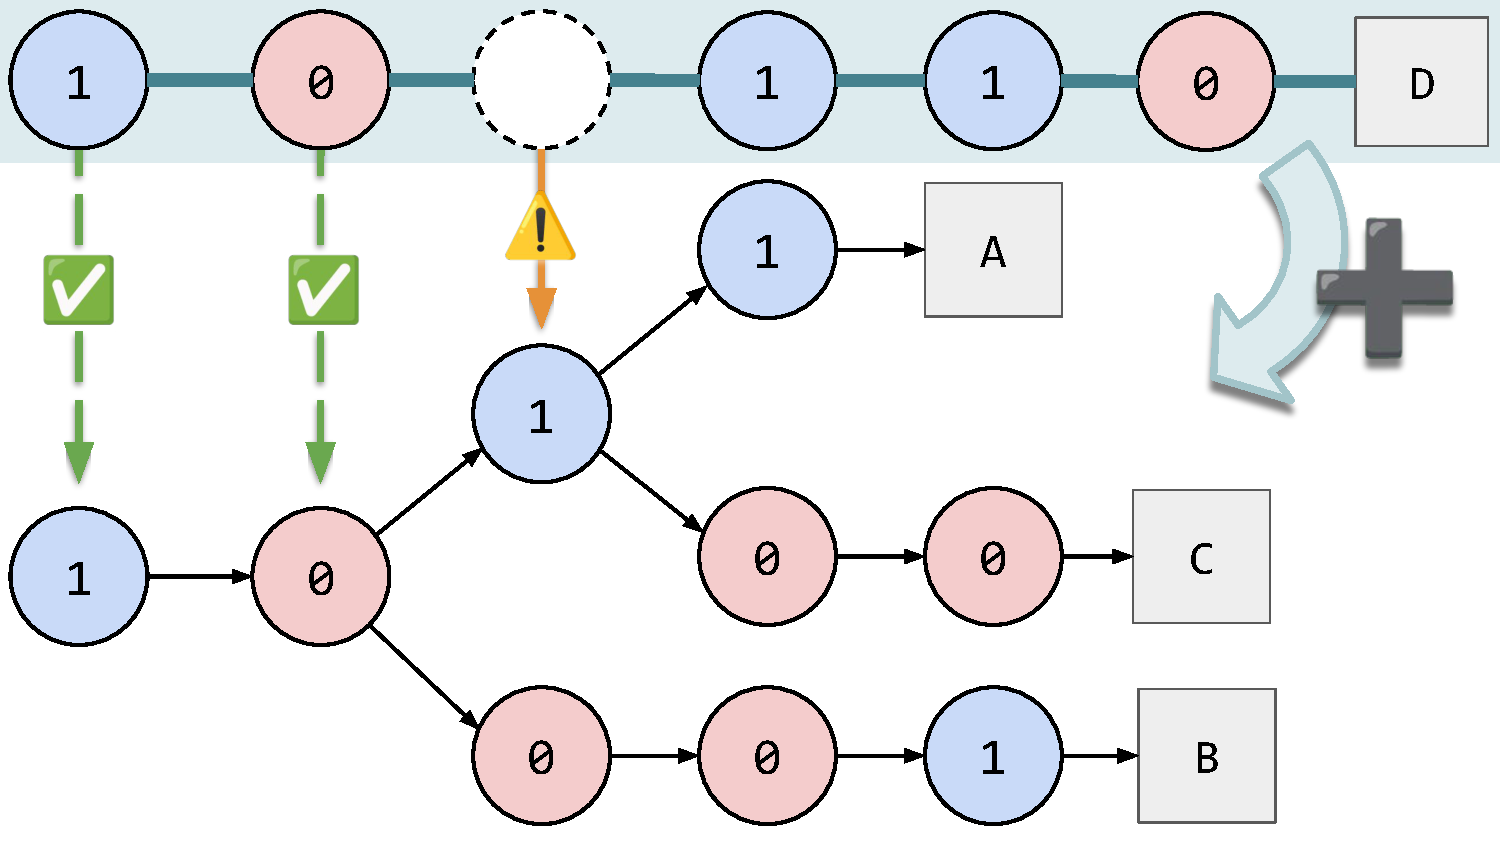
\includegraphics[width=\linewidth]{img/shortcut-algo-diagram-1}
  \subcaption{Preparing to add $D$}
  \label{fig:shortcut-algo-diagram-1}
\end{minipage}
\begin{minipage}{0.32\linewidth}
  \centering
  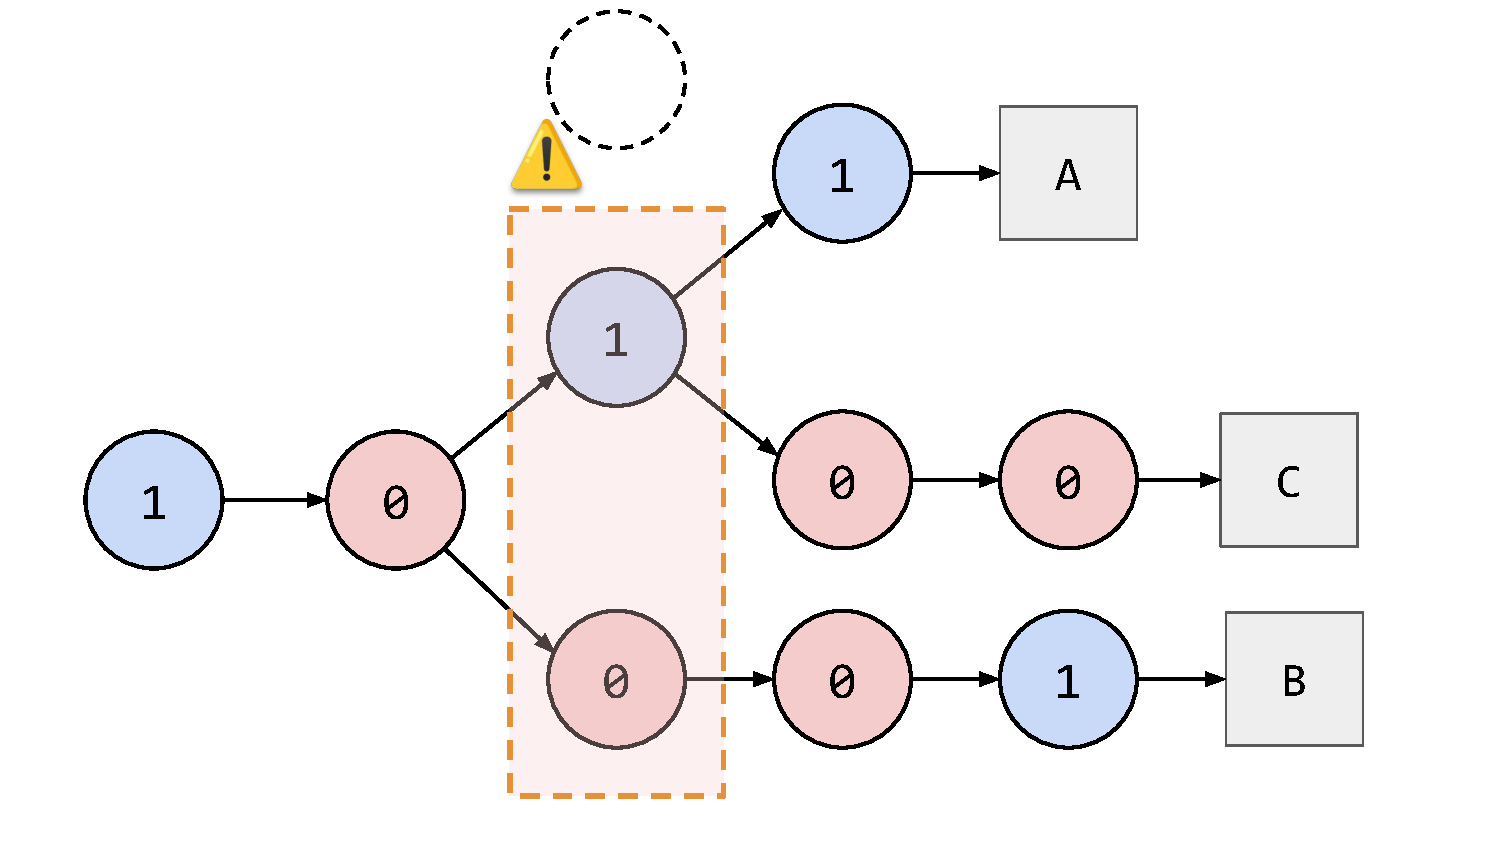
\includegraphics[width=\linewidth]{img/shortcut-algo-diagram-2}
  \subcaption{Encountering dropped marker}
  \label{fig:shortcut-algo-diagram-2}
\end{minipage}
\begin{minipage}{0.32\linewidth}
  \centering
  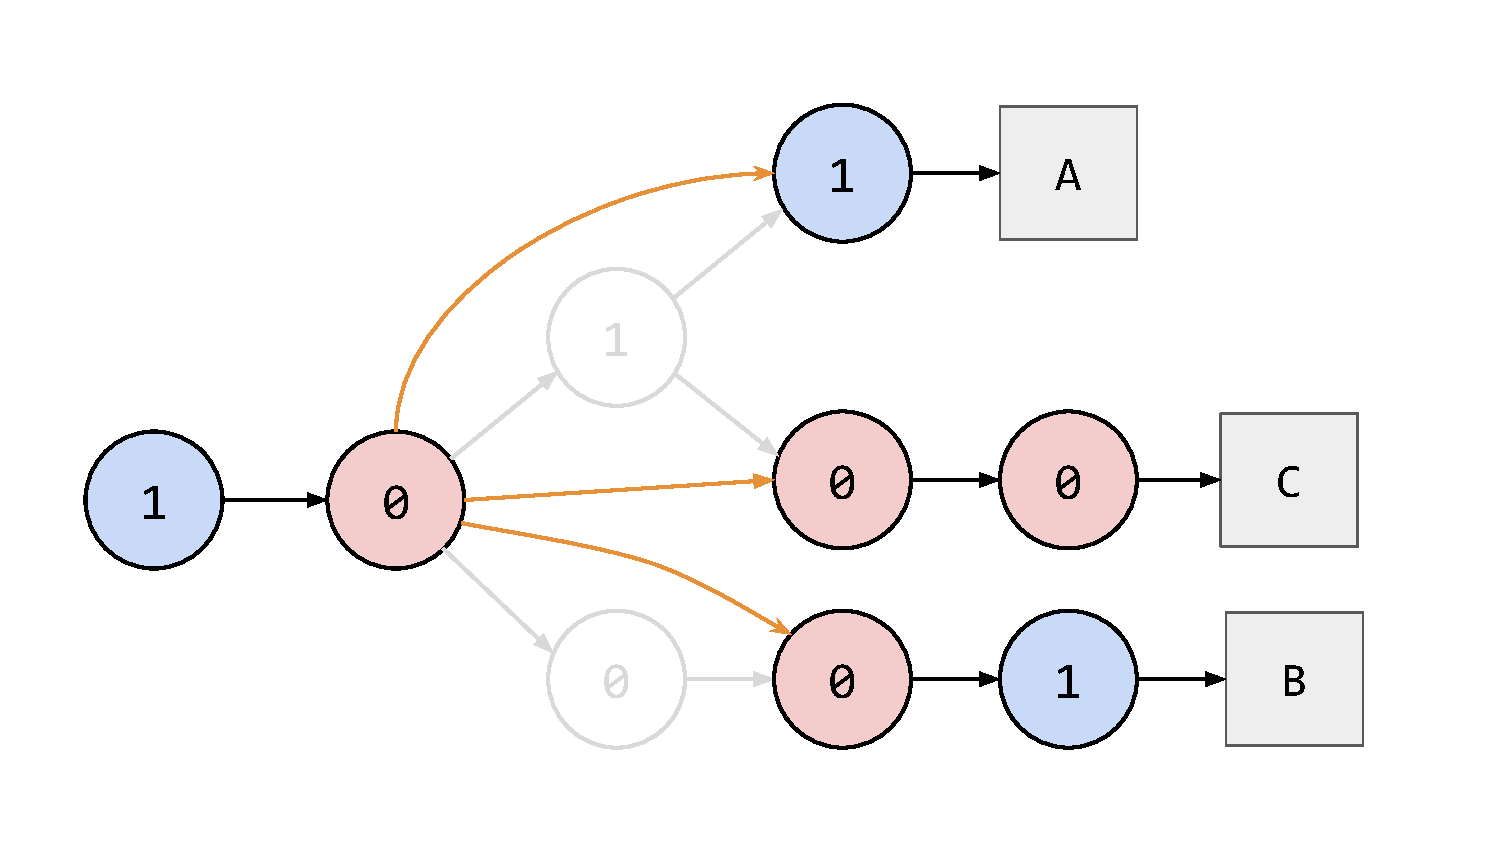
\includegraphics[width=\linewidth]{img/shortcut-algo-diagram-3}
  \subcaption{Building shortcuts}
  \label{fig:shortcut-algo-diagram-3}
\end{minipage}
\begin{minipage}{\linewidth}\par\end{minipage}
\begin{minipage}{0.32\linewidth}
  \centering
  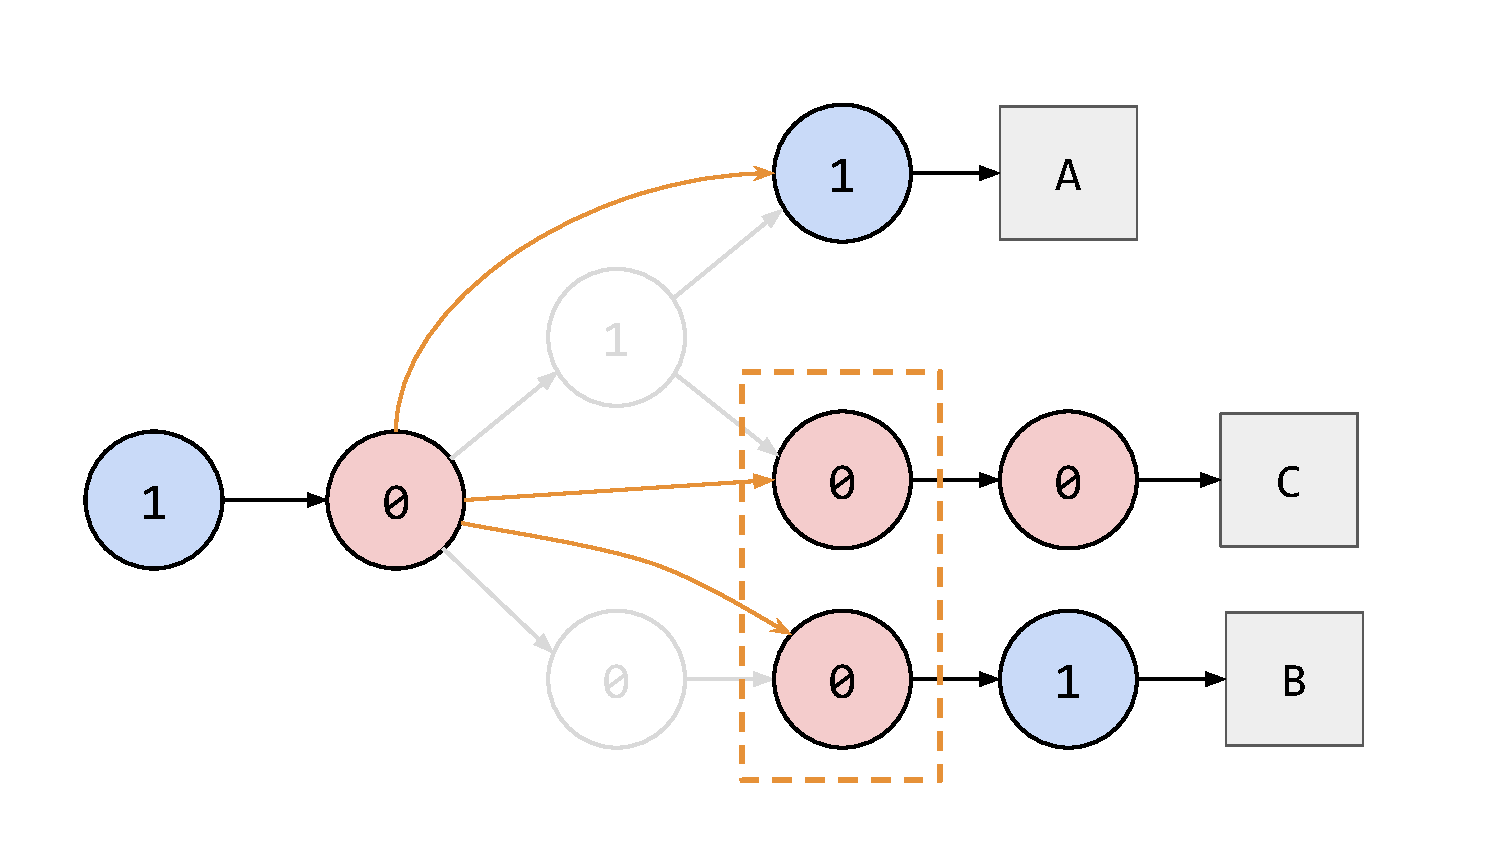
\includegraphics[width=\linewidth]{img/shortcut-algo-diagram-4}
  \subcaption{Indistinguishable nodes}
  \label{fig:shortcut-algo-diagram-4}
\end{minipage}
\begin{minipage}{0.32\linewidth}
  \centering
  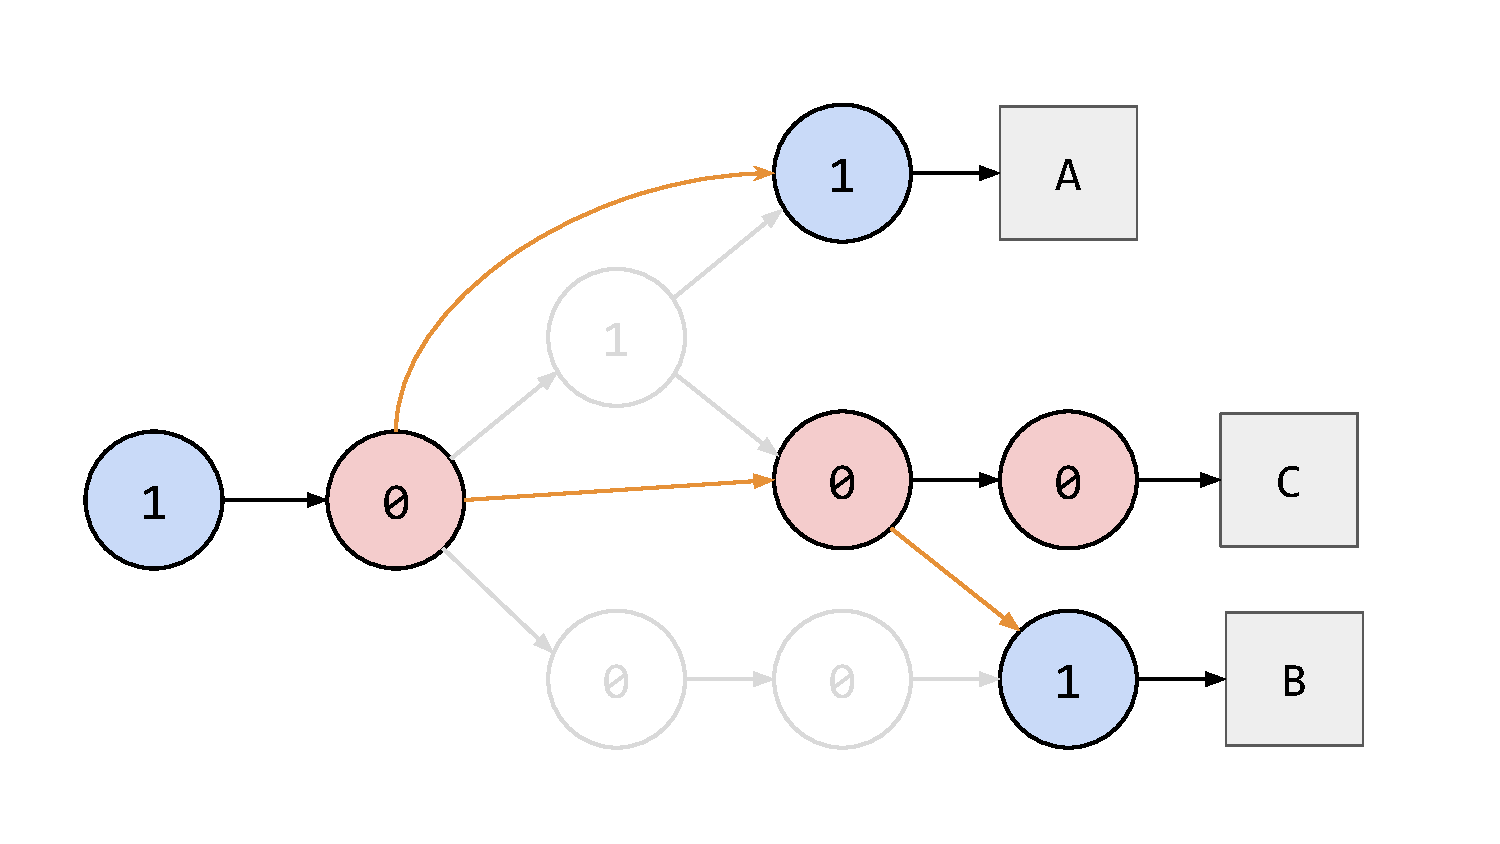
\includegraphics[width=\linewidth]{img/shortcut-algo-diagram-5}
  \subcaption{Collapsing redundant shortcuts}
  \label{fig:shortcut-algo-diagram-5}
\end{minipage}
\begin{minipage}{0.32\linewidth}
  \centering
  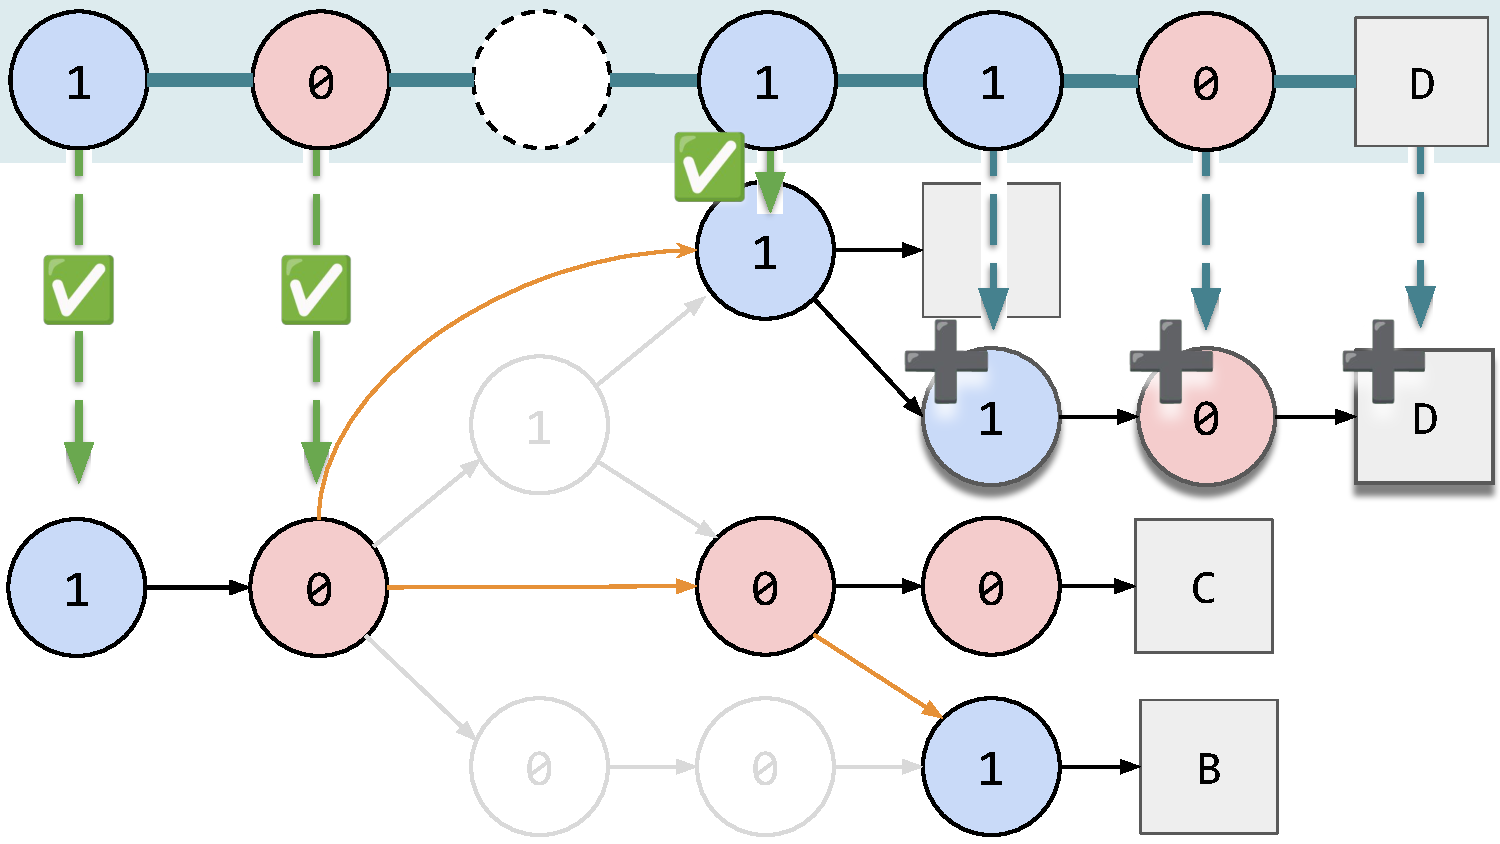
\includegraphics[width=\linewidth]{img/shortcut-algo-diagram-6}
  \subcaption{Organism $D$ added}
  \label{fig:shortcut-algo-diagram-6}
\end{minipage}
\end{minipage}
\begin{minipage}{0.24\linewidth}
\caption{%
\textbf{Trie-consolidation procedure for proposed shortcut algorithm.}
\small
A dropped hereditary marker is encountered while extending trie with genome $D$ (panel \ref{fig:shortcut-algo-diagram-2}).
All subsequent-added genomes will also have dropped markers at this position, so corresponding trie nodes may be bypassed by ``shortcut'' connections (panel \ref{fig:shortcut-algo-diagram-3}).
Note that bypassed trie structure is retained (``grayed-out'' nodes), so corresponding phylogenetic structure remains when reconstruction is finalized.
In a final step, shortcuts leading to identical nodes are further consolidated (panels \ref{fig:shortcut-algo-diagram-4} and \ref{fig:shortcut-algo-diagram-5}).
}
\label{fig:algo-diagram}
\end{minipage}
\vspace{-1.5em}
\end{figure*}


We present a modification of Algorithm~\ref{alg:old} where we replace the best path search in line 9 with a more intelligent consolidation step to deal with missing ranks.
The main idea of this algorithm is to realize that, as previously stated, once data from a specific rank is no longer included in one organism, it will not be included in any subsequent organisms, meaning that the nodes in the tree corresponding to that rank are no longer useful.
So, by building shortcuts around any nodes that have become irrelevant, we can speed up the reconstruction process for all future nodes, too.

We detect missing information the same way as in the naive trie algorithm: during iteration, we notice that when a child $c$ of the current node $n$ has a rank $r'$ that is less than the current rank $r$ being processed, we know we do not have information for any rank between $r'$ and $r$ for this organism and any subsequent organism (due to sorting by generational depth).
% The key insight to the way we manage this scenario is that, in the big picture, we only care about this child if some of its descendants at rank $r$ have a differentia value $d$.

Extending this idea, we know that information for any rank between $r'$ and $r$ is meaningless (as they all have been deleted for organism $o$ and any subsequent organisms). 
So, we can bypass every one of $n$'s descendants that have a rank less than $r$, as their information is now meaningless.
More clearly, we do this by creating shortcut edges from $n$ to the set of descendants whose rank is at least $r$, but whose parent's rank isn't. For example, see Figure~\ref{fig:algo-diagram}, where we detect a dropped rank in (b) and create shortcut edges in (c), around each descendant with that dropped rank.

However, since some descendants of $n$ may have children with equivalent information (like step (d) in Figure~\ref{fig:algo-diagram}), we may end up with shortcuts from $n$ to effectively indistinguishable nodes (with different original parents but the same differentia value).
This situation can be resolved by essentially `merging' the duplicates by choosing one to keep and creating more shortcut edges from the kept one to the children of the removed one (see step (e) in Figure~\ref{fig:algo-diagram}).

Now, adding any organisms that are missing data from the removed level becomes trivial, as the algorithm can use the newly created shortcuts while skipping the missing information that was hidden by the consolidation step.
We no longer need to look down branches from $n$ because the ``wildcard'' value has been eliminated --- each child of $n$ now has a rank greater than or equal to $r$.
% So, there is no longer a concern of missing information when processing $n$ at rank $r$, and these shortcuts are then used to add any subsequent organisms if need be.
If, at some point in the algorithm, $r$ itself becomes a rank of missing information, additional shortcuts are built according to the same procedure.

\begin{algorithm}[h]
  \begin{algorithmic}[1]
  \small{
    \Function{ConsolidateTree}{tree $T$, node $n$, rank $r$}
      \State $S \gets \{c \in \operatorname{descendants}(n) : \operatorname{rank}(c) \ge r \land  \operatorname{rank}(\operatorname{parent}(c)) < r\}$ 
      \For{$c$ in $S$} 
        \textsc{BuildShortcut}($T$, $n$, $c$)
      \EndFor
      \For{each subset of duplicate\footnotemark nodes $S' \subseteq S$}
        \State $c^* \gets$ an arbitrary element in $S'$ 
        \For{$c' \in S \setminus \{c^*\}$}
          \For{$c$ in $\operatorname{children}(c)$} 
            \State \textsc{BuildShortcut}($T$, $c^*$, $c$)
          \EndFor
          \State \textsc{RemoveShortcut}($T$, $n$, $c'$)
        \EndFor
      \EndFor 
    \EndFunction
    \Function{BuildShortcut}{tree $T$, node $n$, node $c$}
      \State $\operatorname{edges}(T) \gets \operatorname{edges}(T) \cup \{(n, c)\}$
      \State $\operatorname{edges}(T)[(n, c)]\text{.is\_shortcut} \gets \textsc{True}$
    \EndFunction
    \Function{RemoveShortcut}{tree $T$, node $n$, node $c$}
        \State $\operatorname{edges}(T) \gets \operatorname{edges}(T) \setminus \{(n, c)\}$
    \EndFunction
  }
  \end{algorithmic}
  \caption{\textbf{The consolidation step of the shortcut table algorithm.} \small Builds shortcuts for a given node $n$ and collapses duplicate children caused by those shortcuts. Note that \vspace{-1.5em}}
  \label{alg:consolidation}
\end{algorithm}
\footnotetext{nodes $x$ and $y$ are duplicates iff $\operatorname{rank}(x) = \operatorname{rank}(y)$ and $\operatorname{differentia}(x) = \operatorname{differentia}(y)$}

The key to maintaining accuracy lies in the fact that since we retain original trie structure information (as represented by the gray nodes in Figure~\ref{fig:algo-diagram}), we preserve the full detail and granularity of the naive approach.
After the algorithm is run, we can simply use the original trie edges as the inferred phylogenetic tree.
See Algorithm~\ref{alg:consolidation} to see pseudocode for this algorithm.
Details about algorithm implementation are provided in supplemental material \citep{supplemental}.
